% !TeX spellcheck = it_IT

\section{Cos'è lo smart working?}
Il termine \textit{smart working} si riferisce alle nuove modalità lavorative all'interno di \mbox{un'organizzazione}, rese possibili dagli avanzamenti tecnologici e divenute essenziali dalle pressioni economiche, ambientali e sociali. Questi nuovi approcci non nascono da un'idea rivoluzionaria, ma sono il frutto della graduale evoluzione delle nostre pratiche lavorative che sono diventate sempre più collaborative e libere. \\Alla base vi sono tre concetti fondamentali:
\begin{enumerate}
	\item la revisione della leadership e del rapporto tra manager e dipendente, dal controllo alla fiducia;
	\item il ricorso a tecnologie collaborative in sostituzione ai sistemi di comunicazione rigidi;
	\item la riorganizzazione degli spazi di lavoro che vanno oltre le quattro mura di un ufficio.
\end{enumerate}
\newpage
Il risultato dell'applicazione di questi concetti in contesti aziendali è l'aumento della produttività aziendale in un modus operandi che pone al centro dell'attenzione la persona, unificando gli obbiettivi personali e quelli lavorativi. Questo processo responsabilizza il lavoratore che è consapevole e sente propri gli obbiettivi aziendali e non vede più l'organigramma aziendale come una dura piramide da scalare, bensì si sposta l'attenzione dall'organizzazione, centrale nei vecchi modelli, al singolo, cercando di motivarlo e di aumentare la sua dedizione per le attività che svolge.\\
Diminuendo quindi la distanza tra la vita professionale e quella privata, il dipendente valorizza da sè le attività che svolge e risulta più efficiente.
Spesso infatti il termine smart working si utilizza per intendere il telelavoro, la possibilità di lavorare da casa, la creazione di spazi per il coworking o a posti di lavoro più flessibili. Sebbene sia corretto, il concetto va molto oltre queste cose e risiede nella ridefinizione del lavoro per come lo intendiamo.\\ All'atto pratico la sua potenza non risiede nel fatto che gli smart workers non hanno orari d'ufficio rigidi o che non importi dove lavorino, ma nella richiesta del datore di \mbox{lavoro},che vincola il lavoratore unicamente a ottenere i risultati previsti nei tempi stabiliti con il massimo della qualità,. Così facendo il subordinato si sente proprietario del proprio lavoro, autonomo in modalità e tempistiche e viene responsabilizzato, imparando a gestire il suo tempo in modo più intelligente. Il controllo in questo modello lascia spazio alla fiducia nei confronti di un sottoposto. Questa lenta rivoluzione è condotta dai mezzi tecnologici che forniscono più alte possibilità di condivisione fra persone, team e società.\\
Lo smart working favorisce quindi la nascita di nuove figure lavorative, come manager moderni che guidano dei gruppi di professionisti e ne gestiscono le risorse, passando così da controllori a più costruttivi mentori che lavorano sulle individualità della persona, che ne trae vantaggi sia professionalmente che personalmente. \\

\section{Ambienti di lavoro e di formazione virtualizzati}
\subsection{Telepresenza}
 La \textit{telepresenza} è un termine che si riferisce a sistemi che permettono agli utenti di sentirsi in altri luoghi con l'ausilio di un mezzo ingegneristico. Questo vocabolo fu coniato dallo scienziato cognitivo Marvin Minsky nel 1980 facendo riferimento ai sistemi di \textit{teleoperazione} per la manipolazione remota di oggetti fisici.\\
 Siamo già da decenni immersi in sistemi di telepresenza come quelli telefonici, le telecamere e persino registrazioni musicali, ma nessuno ha le potenzialità della realtà virtuale. Prendendo infatti in prestito il concetto di Minsky, possiamo definire nuovamente la VR come "\textit{un'ambiente simulato nel quale un'individuo esperimenta la telepresenza}"\cite{DVR}. Difatti il sistema di percezione umano si è evoluto con interazioni faccia a faccia, ed esse fungono da modello per tutti gli altri tipi di comunicazione, le quali vengono paragonate dal nostro cervello a esperienze in prima persona. Trovarsi dentro una simulazione realistica amplia quindi i livelli di intensità e interazione dei mezzi non immersivi. \\
 Sebbene la realtà virtuale si riferisce all'esperienza di un individuo, condividere lo stesso spazio virtuale con altri utenti accresce il senso di realismo della simulazione, spingendone ancora oltre le potenzialità in ambiti lavorativo o di formazione.  
 
 \subsection{I vantaggi}
 
 La realtà virtuale apre le porte a molteplici benefici in campi lavorativi e formativi. Fornendo una profondissima esperienza di telepresenza il luogo geografico da cui si svolge la propria professione non è più fondamentale, facilitando lo smart working e aumentando la centralità e il benessere della persona nella società.\\
 Si può pensare di entrare in un edificio virtuale e lavorare o incontrare clienti senza il vincolo di essere nello stesso posto reale, utilizzando la comunicazione non verbale assente in altri strumenti di telepresenza. In un ambiente virtualizzato l'esperienza del lavoratore può essere aumentata fornendogli strumenti altrimenti impossibili da utilizzare come traduttori real-time o più semplicemente integrazioni di servizi in modo più intuitivo e naturale. \\
 Questo approccio può essere l'inizio di un radicale cambiamento nei luoghi in cui viviamo e lavoriamo, unificando tutti gli strumenti fisici che occupano spazio, in un unico visore. Un cambiamento simile è stato portato dagli smartphones che hanno incorporato diversi oggetti (agende,orologi,giornali, ecc.) in un unico dispositivo di ridotte dimensioni. La VR, in futuro, potrebbe eliminare gli edifici in cui oggi lavoriamo, lasciando spazio a nuovi luoghi di aggregazione, innescando un processo di \textit{deurbanizzazione} più compatibile con le esigenze del nostro pianeta. \\ 
 
 Un'altro proposto fondamentale della tecnologia è rendere le professioni più sicuri abbassando il rischio di infortuni e morte nel caso di lavori pericolosi. Con l'utilizzo di ambienti virtuali interattivi e di sistemi teleoperazionali, si possono svolgere compiti ad alto rischio, come lo sminamento di un campo, utilizzando un visore ed un robot specializzato che viene controllato a distanza in modo estremamente intuitivo e naturale.\\
 Questo processo di \textit{ludicizzazione} (\textit{gamification}), ovvero l'utilizzo di elementi mutati dai giochi e delle tecniche di game design in contesti esterni ai giochi \cite{Gamification}, può far beneficiare anche la classe operaia delle rivoluzioni tecnologiche di solito riservate a professioni più prestigiose e si propone di risolvere l'alto tasso di disoccupazione tra i giovani videogiocatori \cite{Leisure}.\\
 L'adozione di questo approccio porterebbe anche vantaggi socio economici come la riduzione dell'inquinamento dovuto agli spostamenti tra le abitazioni e i luoghi di lavoro.  \cite{POL}
 \begin{figure}[H]
 	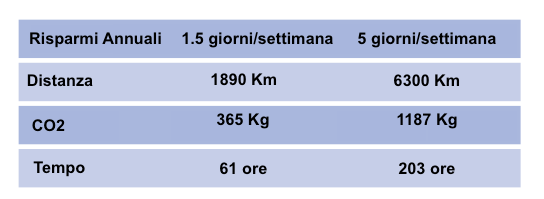
\includegraphics[width=0.65\textwidth]{figure/PolData}
 	\centering
 	\caption{I dati raccolti da uno studio dell'Università di Oxford sui risparmi ottenuti grazie al telelavoro nel Regno Unito.}
 \end{figure}
\newpage
Le potenzialità più grandi della realtà virtuale risiedono però in campo formativo. Bambini e ragazzi impossibilitati a raggiungere un luogo di studio possono comunque avere accesso ad un'istruzione. Nonostante i sistemi immersivi offrano strumenti unici ed estremamente utili, allo stesso tempo tagliano i costi di formazione professionale evitando anche quelli di eventuali errori commessi da lavoratori inesperti. Questi due aspetti raggiungono l'apice in campi come la medicina, in cui sempre più applicazioni VR vengono utilizzate per insegnare a giovani dottori come portare a termine un'operazione chirurgica o come effettuare una diagnosi esplorando l'interno di un organo malato. \\
Altri campi che beneficerebbero della virtualizzazione sono le aree di ricerca scientifiche. Sempre più spesso infatti sono richiesti per l'insegnamento e la formazione simulatori molto costosi o relazioni geometriche in strutture di dati complesse difficili da visualizzare.  La realtà aumentata è utile per l'insegnamento pratico, perché le abilità imparate nel mondo virtuale realistico possono essere applicate al mondo reale in modo intuitivo.\\
Un'aspetto meno pratico, ma più psicologico su diversi ricercatori stanno studiando è il  collegamento tra empatia e realtà virtuale. Se infatti consideriamo ambienti estremamente realistici, costruiti seguendo una fedele mappatura o con l'utilizzo di camere panoramiche, è possibile considerare un notevole aumento nell'empatia stimolata in un individuo che vive un'esperienza in prima persona. Vivere la guerra in Siria, un giorno  nella cella d'isolamento in una prigione di massima sicurezza o nel corpo del sesso opposto sono alcune esperienze virtuali che più hanno scosso in modo empatico gli utenti,
questo a dimostrazione di quanto può essere immersiva questa tecnologia.
Sempre più organizzazioni stanno cambiando il loro modo di intendere il lavoro e la formazione, puntando su simulazioni in realtà virtuale incrementandone il mercato e innescando così un'ulteriore accelerazione dell'avanzamento tecnologico di questo nuovo mezzo. 
\begin{figure}[H]
	\includegraphics[width=0.65\textwidth]{figure/investimenti}
	\centering
	\caption{I dati raccolti da uno studio dell'Università di Oxford sui risparmi ottenuti grazie al telelavoro nel Regno Unito.}
\end{figure}

\section{Limiti}

Nonostante l'elevato potenziale della realtà virtuale in questi settori, l'adozione di queste nuove tecnologie sarà lento. I dispositivi che abbiamo a disposizione comportano alti prezzi e non vi sono ancora abbastanza applicazioni personalizzate che soddisfino le unicità dei vari settori in cui andrebbero ad operare. La principale funzione dei sistemi VR, ovvero quella di sovrapporsi agli organi di senso della persona, è spesso anche la causa principale della diffidenza nei confronti di questo nuovo mezzo. \\
Infatti, a differenza dei vecchi media (libri, radio, televisioni, ecc.) la realtà virtuale può causare stanchezza e nausea definita proprio \textit{VR sickness}. Spesso il malessere può essere provocato da un hardware difettoso o da uno sviluppatore che ha sottovalutato gli effetti collaterali della VR. Chi sviluppa il software infatti deve avere come prima priorità la salute dell'utente, per questo motivo l'utilizzatore finale deve essere considerato come parte integrante del sistema. In molti casi la stanchezza sopraggiunge per il costante lavoro del cervello nel ricalibrare gli stimoli sensoriale incoerenti con la realtà che possono anche condurre a giramenti di testa. Essendo un'attività fisica in cui tutto il corpo è coinvolto, interazioni scomode all'interno dell'applicazione,come  il continuo movimento delle braccia nell'esperienza virtuale per interagire con l'ambiente, possono portare ad effetti indesiderati come le \textit{gorilla arms}, termine poco tecnico per definire la sensazione per la quale gli utenti non sopportano più il peso delle proprie braccia estese. Alcuni degli effetti collaterali devono ancora essere risolti, altri si formano con l'aggiunta di nuove funzionalità o componenti hardware.\\
Purtroppo anche con i migliori visori e con software di alta qualità una persona può reagire negativamente ad un'esperienza in realtà virtuale. ****Un fattore predisponente può essere l'etnia. Michael Sivak e Brandon Schoettle dell'University of Michigan hanno infatti dimostrato che è statisticamente più probabile per una persona asiatica soffrire della sopra citata VR sickness rispetto ad individui caucasici.

\begin{figure}[H]
	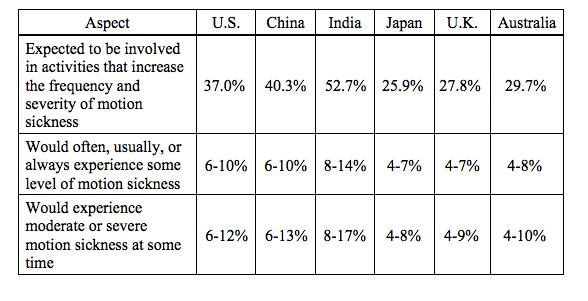
\includegraphics[width=0.65\textwidth]{figure/motionsickenss2}
	\centering
	\caption{I dati raccolti da uno studio dell'Università di Oxford sui risparmi ottenuti grazie al telelavoro nel Regno Unito.}
\end{figure}

In conclusione bisognerà aspettare sistemi meno ingombranti, più economici e un maggior numero di sviluppatori esperti per poter diffondere e sfruttare al massimo le potenzialità della realtà virtuale. Citando Dave Jones, il creatore del primo videogioco della serie Grand Theft Auto, "La realtà virtuale è ancora all'età della pietra" \cite{VRStone}. 

